% !TeX spellcheck = en_GB
\section{Surface snowfall accumulation}
The surface accumulation is a good point to start to see, if the retrieved snowfall amounts at the surface catch the boundary condition as of the double fence. Precipitation amount at the surface are shown in \Cref{fig:sfc_acc}. The figures are representing the observed surface precipitation accumulation in \SI{}{\mm} for \SI{48}{\hour}. Accumulation, measured by the double fence are presented as purple hexagons. Retrieved surface snowfall amount in dash-dotted orange. The ten \SI{48}{\hour} forecast ensemble members are lines in black and grey, the deterministic and its perturbed ensemble members, respectively. The blue dashed line shows the ensemble mean of all ten members. Since the deterministic and the first ensemble member are having values every hour and the other perturbed members only every three hours, shows the ensemble mean the precipitation amount at 0\SI{0}{\UTC}, \SI{3}{\UTC}, $\ldots$, \SI{21}{\UTC}, \SI{24}{\UTC}, $\ldots$. 
Underneath is the associated \SI{10}{\minute} average wind of the last hour from the \SI{10}{\metre} weather mast at Haukeliseter. 
%%% image surface accumulation %%%%%%%%%%%%%%%%%%%%%%%%%%%%%%%%%%%%%
% !TeX spellcheck = en_GB
%\begin{landscape}
\begin{figure}[t!]
	\centering
	% 21/12
	\begin{subfigure}[t]{0.49\textwidth}		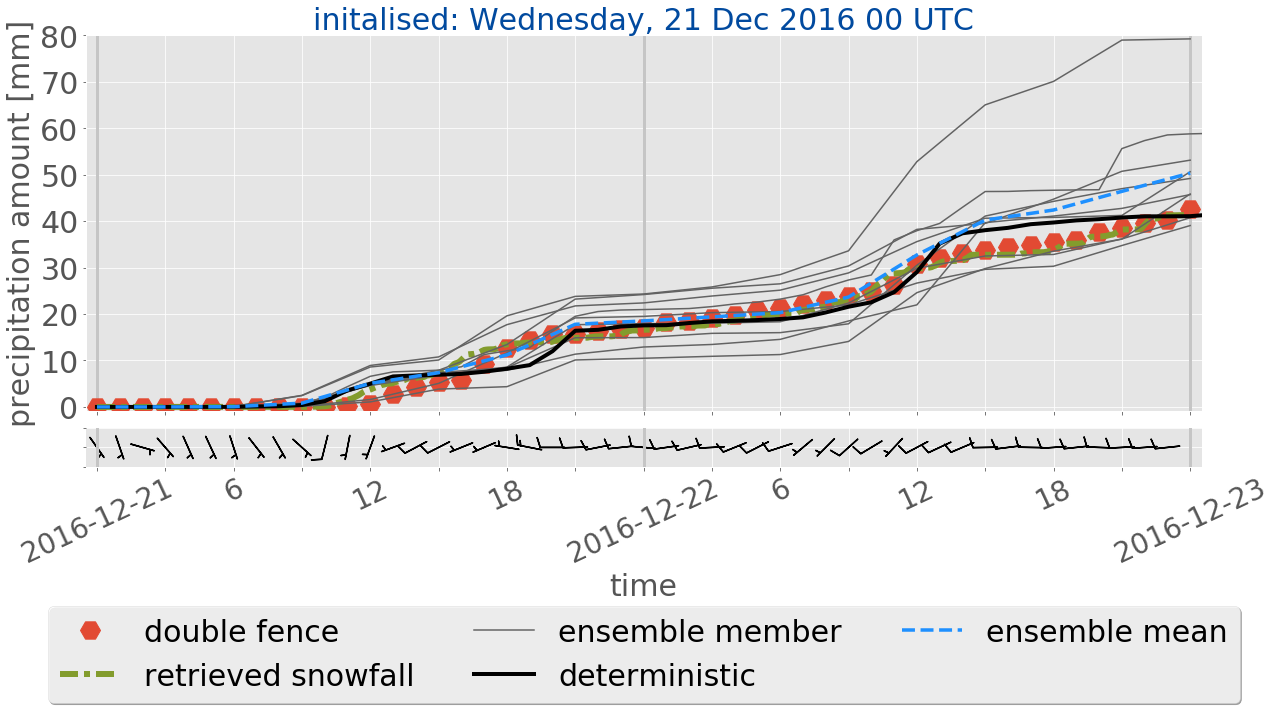
\includegraphics[trim={3.cm 2.6cm 2.cm 1.9cm},clip,width=\textwidth]{./fig_sfc_acc/acc_wind_20161221_00}
		\caption{}\label{fig:sfc_acc21}
	\end{subfigure}
	% 22/12
	\begin{subfigure}[t]{0.49\textwidth}		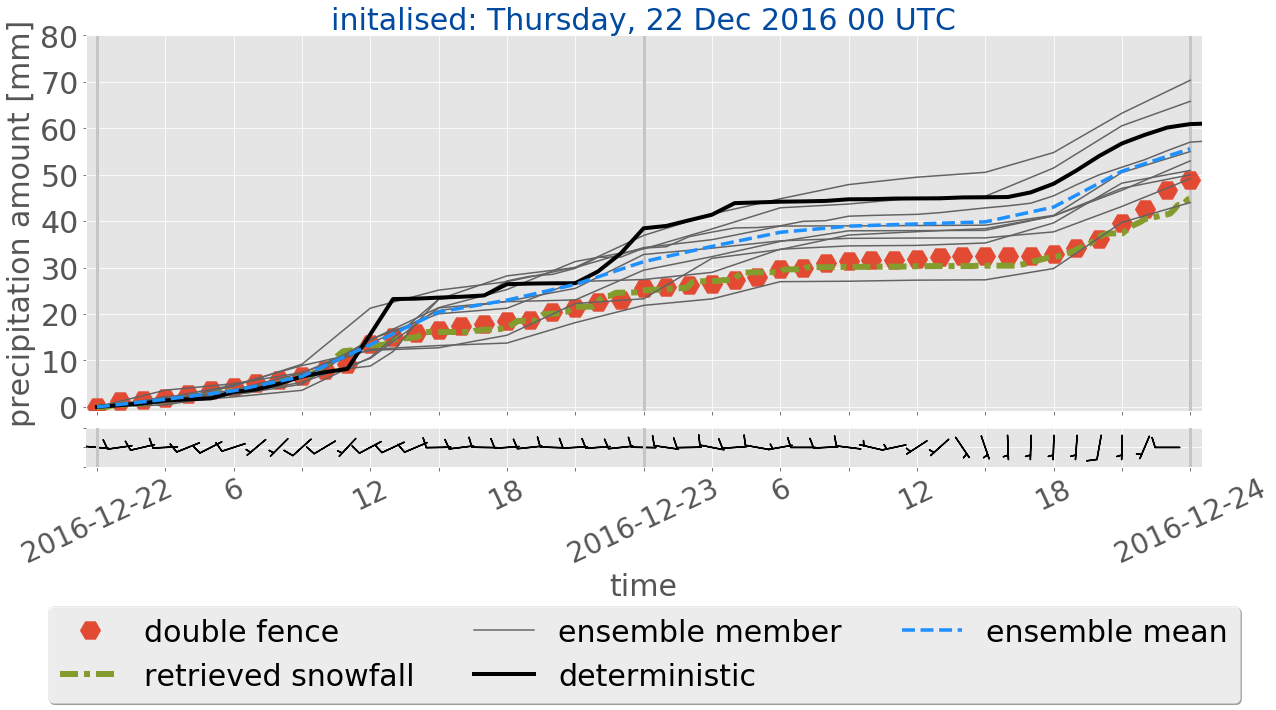
\includegraphics[trim={3.cm 2.6cm 2.cm 1.9cm},clip,width=\textwidth]{./fig_sfc_acc/acc_wind_20161222_00}
		\caption{}\label{fig:sfc_acc22}
	\end{subfigure}
	%	\end{figure}
	%   \begin{figure}\ContinuedFloat
	% 23/12
	\begin{subfigure}[t]{0.49\textwidth}	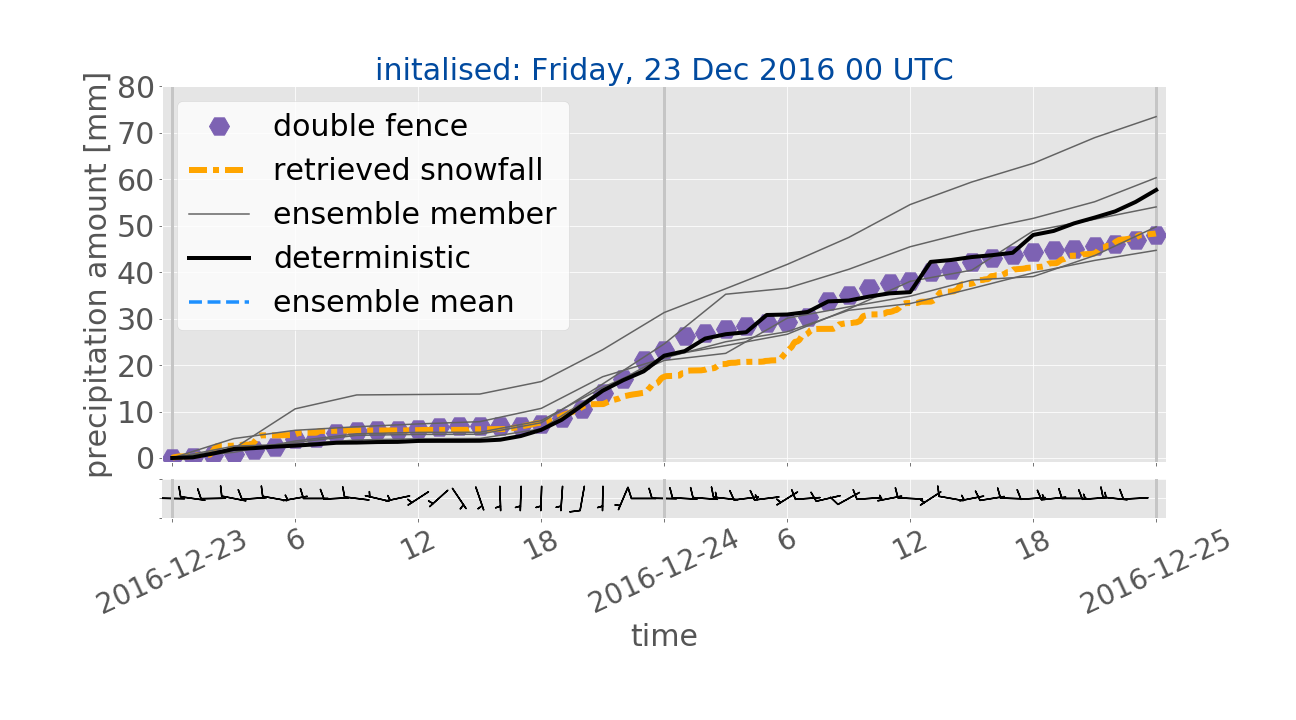
\includegraphics[trim={3.cm 2.6cm 2.cm 1.9cm},clip,width=\textwidth]{./fig_sfc_acc/acc_wind_20161223_00}
		\caption{}\label{fig:sfc_acc23}
	\end{subfigure}
	% 24/12
	\begin{subfigure}[t]{0.49\textwidth}			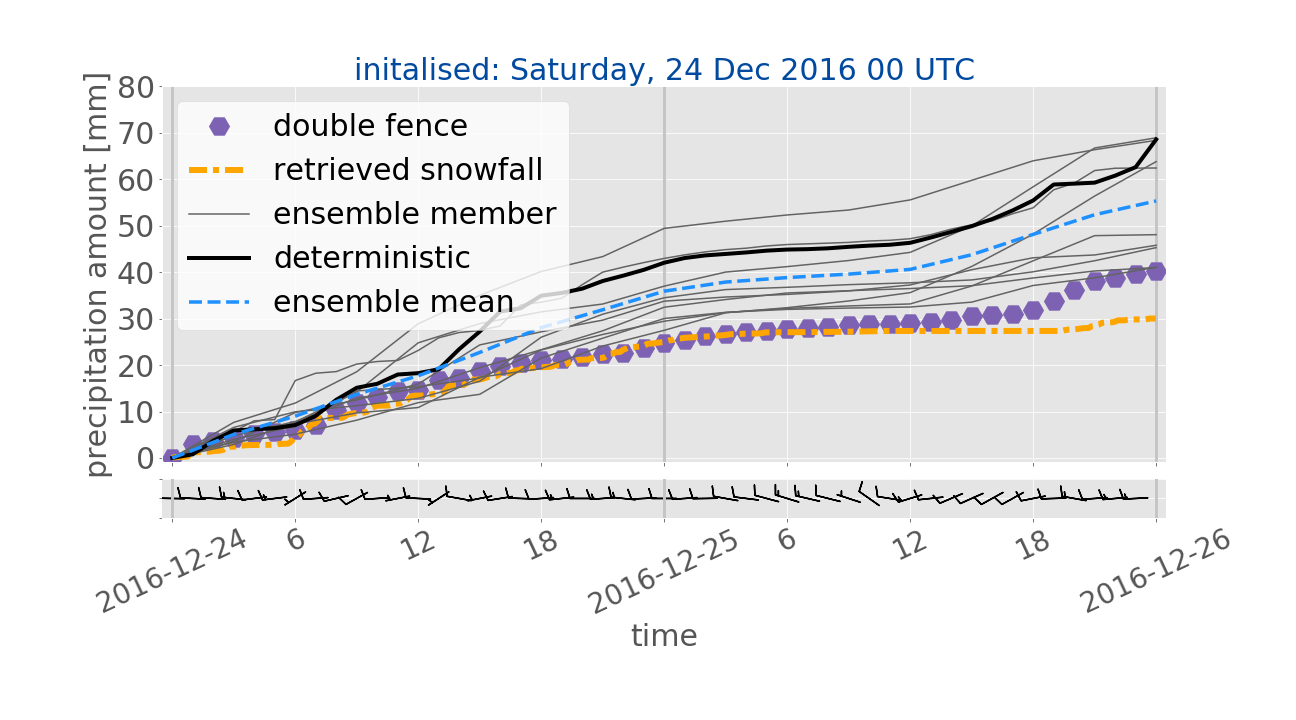
\includegraphics[trim={3.cm 2.6cm 2.cm 1.9cm},clip,width=\textwidth]{./fig_sfc_acc/acc_wind_20161224_00}
		\caption{}\label{fig:sfc_acc24}
	\end{subfigure}
	% 25/12
	\begin{subfigure}[t]{0.49\textwidth}
		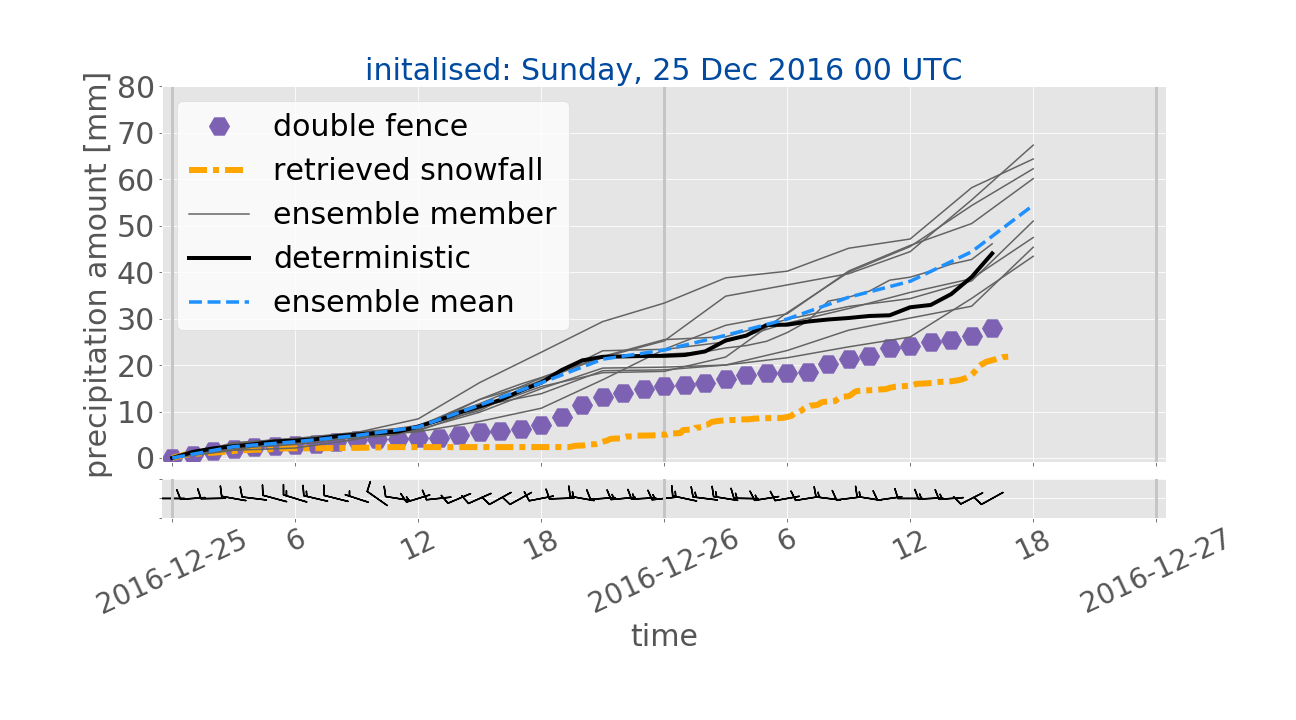
\includegraphics[trim={3.cm 2.6cm 2.cm 1.9cm},clip,width=\textwidth]{./fig_sfc_acc/acc_wind_20161225_00}
		\caption{}\label{fig:sfc_acc25}
	\end{subfigure}
	% 26/12
	\begin{subfigure}[t]{0.49\textwidth}	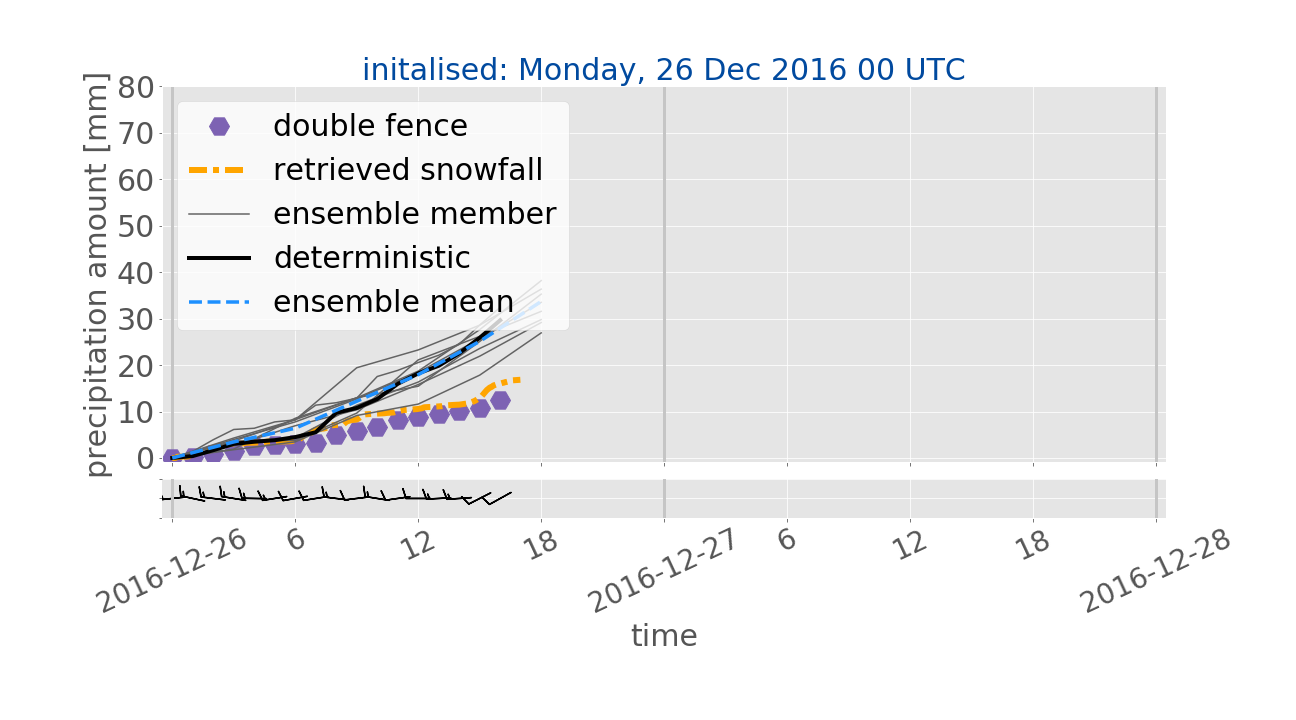
\includegraphics[trim={3.cm 2.6cm 2.cm 1.9cm},clip,width=\textwidth]{./fig_sfc_acc/acc_wind_20161226_00}
		\caption{}\label{fig:sfc_acc26}
	\end{subfigure}
	\caption{Surface snowfall accumulation. Representing the values from the double fence in purple, hexagons; optimal estimation retrieval output at snow layer height \SI{800}{\metre} in dash-dotted orange; and ensemble member deterministic forecast, initialised at 0\SI{00}{\UTC} in black and its nine perturbed ensemble members in grey. The ensemble mean of all ten members is shown in blue dashed.  Underneath are the associated last \SI{10}{\minute} average wind from the weather mast at \SI{10}{\metre} height. }\label{fig:sfc_acc}
\end{figure}



%%%%%%%%%%%%%%%%%%%%%%%%%%%%%%%%%%%%%%%%%%%%%%%%%%%%%%%%%%%%%%%%%%%%%%%%%%
\noindent
In general show the \SI{48}{\hour} surface accumulation in \Cref{fig:sfc_acc21,fig:sfc_acc22,fig:sfc_acc23} a good agreement between the foretasted values and the retrieved snowfall amount when comparing to the double fence. \SI{24}{\dec} and \SI{25}{\dec} show a large disagreement between the observations and the model forecast. \\
The surface accumulation initialised on the \SI{21}{\dec} 0\SI{0}{\UTC} has one ensemble member overestimating the precipitation amount after \SI{33}{\hour} forecast time. Otherwise, agree all three systems well with each other and the perturbed ensemble members are equally distributed around the deterministic forecast.
\\
On \SI{22}{\dec} (\Cref{fig:sfc_acc22}) fit the ensemble mean relatively well to the observed surface accumulation. Remarkable is the fact, that the perturbed ensemble members are not equally spread around the deterministic forecast and that the deterministic is predicting more surface accumulation. 
\\
When too few ensemble members were present, then no ensemble mean is calculated as for \SI{23}{\dec}. \Cref{fig:sfc_acc23} shows a well agreement between the double fence observations and the deterministic forecast. Here, for the first time measures the retrieved surface snowfall accumulation less than for the double fence.
\\
\Cref{fig:sfc_acc24} indicates an overestimation of surface snowfall already after \SI{13}{\hour} forecast time, when initialised on \SI{24}{\dec}. The deterministic forecast in solid black is much higher and increases faster than the observations. A higher value of approximately \SI{15}{\mm} can be seen when compared to the surface measurements. This difference remains almost constantly over the forecast time. Since the double fence is exposed to wind one might assume a precipitation under-catch at the surface, but by comparing the \SI{10}{\minute} average wind at \SI{13}{\UTC} it shows not to be a relationship between surface snowfall and wind, rather a forecasting error in MEPS. 
\\
On the \SI{26}{\dec} the MRR did not work after approximately \SI{17}{\UTC} and therefore only values after \SI{17}{\UTC} are not comparable. \Cref{fig:sfc_acc25} shows a similar overestimation of MEPS compared to the surface observations. After \SI{12}{\hour} forecast time the ensemble members overestimate the surface accumulation. Also, the retrieved snowfall accumulation seems to be too little over the entire period, when it starts to precipitate more around \SI{18}{\UTC} on the \SI{25}{\dec}. This might be, because the optimal estimation retrieval does not account for liquid precipitation as the double fence gauge measures liquid and solid precipitation, this will be further discussed in \Cref{sec:2512}.

%%%% DISCUSSION of sfc accumulation %%%%%%%%
\textcolor{red}{DISCUSS! Why is the surface accumulation predicted better for the first days and not too well for the \SIlist{24;25}{\dec}? From Introduction, since excluded: \\
	During the first few days the ensemble outputs cover the amount of snow good in comparison to the double fence observations.
	The spread of the ensemble members around the control run fits as well to the observations for this time period. But, for an initialisation on the \SI{24}{\dec}, \SI{18}{\UTC} one can see that  MEPS over estimates the amount of snow accumulation. It is even more pronounced with the initialisation on the \SI{25}{\dec}, \SI{18}{\UTC} (compare \Cref{fig:acc25}). 
	\\
	This can have different reasons. One of them can be that the large scale weather situation was more predictable for the first four days (\Cref{fig:acc20,fig:acc21,fig:acc22,fig:acc23}). 
	According to \cite{muller_arome-metcoop:_2017} are strong precipitation events better predicted with MEPS than ECMWF (European Centre for Medium-Range Weather Forecasts). On the other side, \cite{muller_arome-metcoop:_2017} states, that an overestimation appears, where the precipitation event (\SI{12}{\hour} accumulation) is less than \SI{10}{\mm}. This is not the case for the time period \SIrange{21}{26}{\dec} (compare \Cref{fig:DecObs}), where the daily precipitation exceed \SI{10}{\mm} every day. The question arises why MEPS covers the high amount of snow accumulation on the \SI{24}{\dec} but forecasts \SI{24}{\hour} prior to \SIlist{25;26}{\dec} are not covering the predicted amount of accumulation!}